À partir du cahier des charges de la première partie, nous savons déjà comment mettre en place tout ce qui 
  n'est pas la simulation en elle-même. Car au départ, il n'y a pas encore d'expériences, ni de résultats, on ne peut donc que réaliser ce dont on est sûr d'avoir besoin. Malheureusement, dans la plupart des cas, c'est la chose de plus complexe à réaliser.
  Par exemple, il faut créer un menu, c'est évident. Or la SDL ne propose rien de tel. Nous allons donc créer notre propre menu, de manière à pouvoir le modifier facilement au cours du développement et le réutiliser dans des programmes ultérieurs. Le menu est en fait un «~module~». L'idéal dans la programmation de nos jours, est non pas d'avoir le code avec le moins de lignes possibles, mais le code le plus lisible et le plus modulaire. Chaque module doit être indépendant des autres, être facilement modifiable et extensible.
  Voici la liste des modules qu'il faut absolument créer : 
  \begin{itemize}
    \item Le menu
    \item La boite de pétri
    \item La cellule
    \item L'affichage\footnote{Qui simplifie l'utilisation de la SDL, par exemple une fonction «~dessineCellule~» qui exécute automatiquement une liste d'instruction SDL}
  \end{itemize}
  
  Dans chaque module, il y aura différents éléments : 
    \begin{itemize}
      \item Des fonctions
      \item Des variables gobales
      \item Des Classes ou des Structures
    \end{itemize}
  Une classe ou une structure est un patron, une définition formelle d'un nouveau type.
  Après les types classiques comme les nombres ou les lettres, on a la possibilité de créer
  des combinaisons de type (on peut aussi combiner des structures). Tout ceci est définit 
  clairement dans l'annexe \ref{DefStruct} pour les structures, et \ref{DefPOO} pour les
  classes.
  
  Il faut impérativement que chaque module soit bien configurable, adaptable, réutilisable et modifiable facilement, car nous n'avons pour l'instant encore aucune idée des valeurs exactes de la simulation, il faut donc prévoir tous les cas impérativement.
  
  \begin{figure}[H]
		\centering
		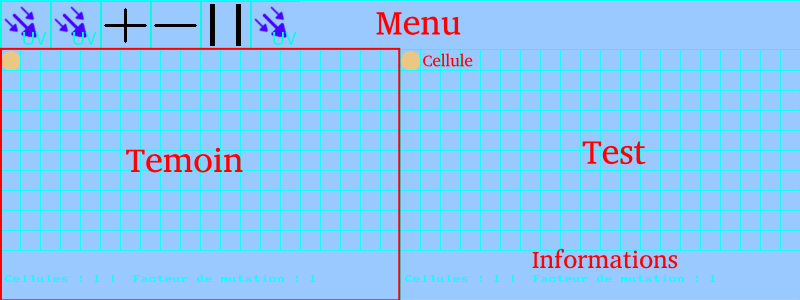
\includegraphics[width=20em]{Images/capture.png}
		\caption{Première vue du programme}
	\end{figure}
